\subsection{Diseño Módulo 4}

En esta sección se deifine la tanto el diagrama de secuencia el cual indica la interacción del usario con el sistema, así como 
las pagínas web que se muestran en este módulo.

\subsubsection{Diagrama de secuencia}

A continuación en la \ref{fig:Sec1} se muestra el diagrama de secuencia del módulo 4, 
el cual indica la interacción del usuario con el sistema.

 \begin{figure}[htbp]
    \centering
    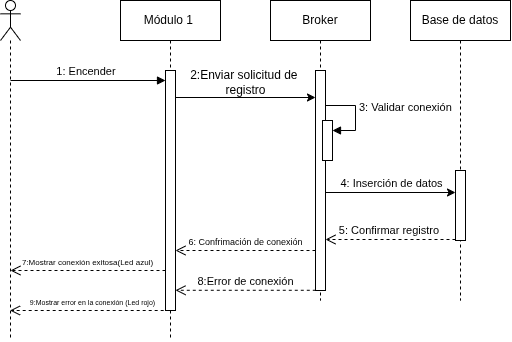
\includegraphics[width=.9\textwidth]{./UML/Modulo4/vertical1.drawio.png}
    \caption{Secuencia de interacción del usuario con el sistema en el módulo 4}
    \label{fig:Sec1}
    \end{figure} 

\subsubsection{Pantallas del sistema}

A continuación, se presentan y describen las interfaces del administrador,productor inicial y raíz correspondientes al Módulo 4.

En la \cref{fig:Main4} se ilustra la pantalla principal que ambos usuarios pueden ver,
la cual funciona como punto de acceso e integra los componentes de navegación hacia las 
demás secciones del sistema. Por su parte, en la \cref{fig:Login4} y en la \cref{fig:Recuperar4} 
se observan las pantallas de inicio de sesión y de recuperación de contraseña, respectivamente. 


\begin{figure}[htb]
\centering
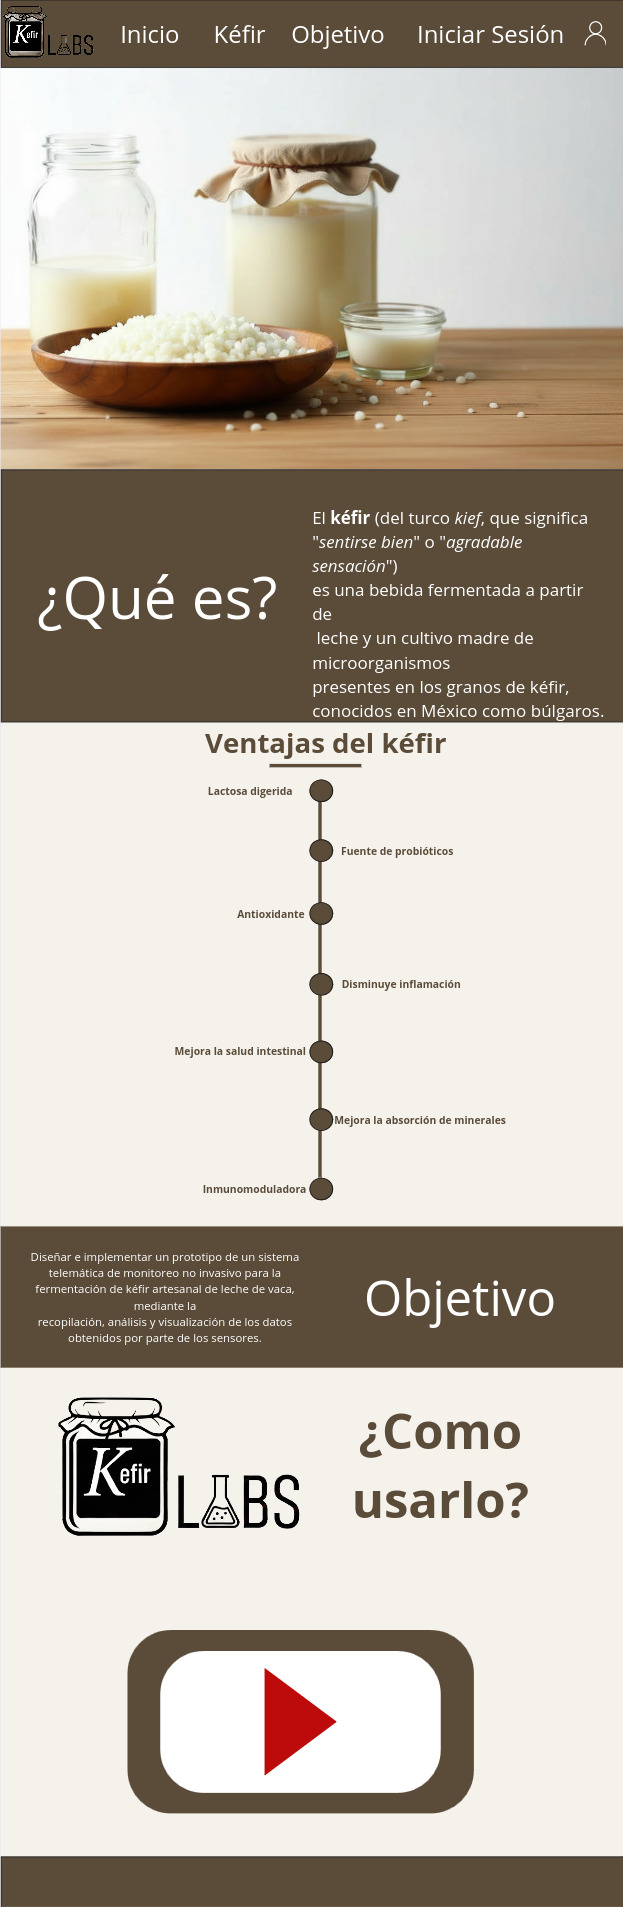
\includegraphics[width=0.5\textwidth]{./UML/Modulo4/Pagina/Main.jpg}
\caption{Pantalla principal del módulo 4.}
\label{fig:Main4}
\end{figure}


\begin{figure}[htb]
\centering
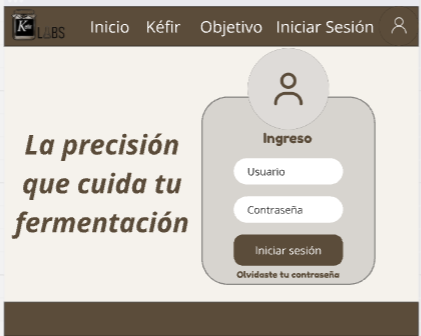
\includegraphics[width=0.8\textwidth]{./UML/Modulo4/Pagina/login.png}
\caption{Pantalla de inicio de sesión del módulo 4.}
\label{fig:Login4}
\end{figure} 

\begin{figure}[htb]
\centering
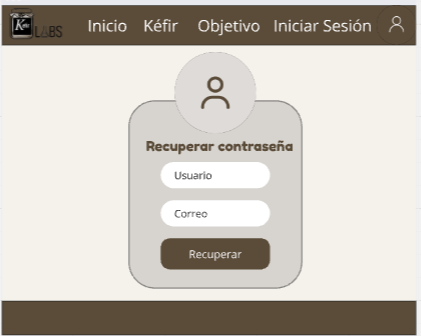
\includegraphics[width=0.8\textwidth]{./UML/Modulo4/Pagina/recuperar.png}
\caption{Pantalla de recuperación de contraseña del módulo 4.}
\label{fig:Recuperar4}
\end{figure} 


\subsubsection{Secuencia de páginas web productor inicial y raíz}

El sistema tiene dos tipos de usuarios, el productor inicial y el productor raíz, 
por lo que una vez autenticado el usuario, el sistema despliega la pantalla de bienvenida mostrada en
la \cref{fig:InicialUsusario}. Al acceder a la pestaña de fermentación, 
si no existe ningún proceso activo, se presenta la pantalla de espera
ilustrada en la \cref{fig:EsperaInicial}. 
En caso de que se encuentre un proceso en curso bajo el modo de monitoreo, 
se visualiza la interfaz presentada en la \cref{fig:MonitoreoInicial}. 
Asimismo, si el proceso se ejecuta en modo de prueba, 
se muestra la pantalla de la \cref{fig:PruebaInicial}, 
en la cual el microcontrolador realiza exclusivamente la adquisición de los datos de la fermentación 
sin someterlos al análisis de datos.

Por otro lado, al seleccionar la pestaña del árbol principal,
la interfaz del árbol genealógico adapta su visualización según el perfil del
usuario: si se trata de un productor inicial, 
se despliega la pantalla de la \cref{fig:ArbolPrincipal}, 
mientras que para un productor raíz se muestra la interfaz de la \cref{fig:ArbolRaiz}. 
Finalmente, el acceso a la pestaña de historial despliega la pantalla presentada 
en la \cref{fig:Historial}.

\begin{figure}[htb]
\centering
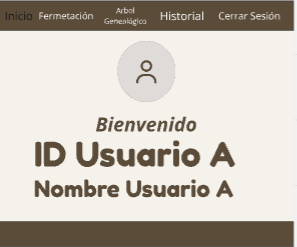
\includegraphics[width=0.8\textwidth]{./UML/Modulo4/Pagina/inicialususario.png}
\caption{Pantalla de inicio de ambos productores.}
\label{fig:InicialUsusario}
\end{figure} 


\begin{figure}[htb]
\centering
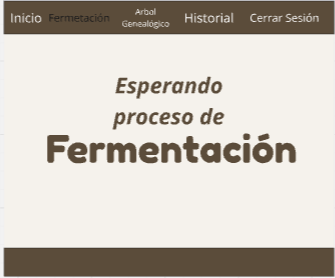
\includegraphics[width=0.8\textwidth]{./UML/Modulo4/Pagina/espera.png}
\caption{Pantalla de espera del productor inicial.}
\label{fig:EsperaInicial}
\end{figure} 

\begin{figure}[htb]
\centering
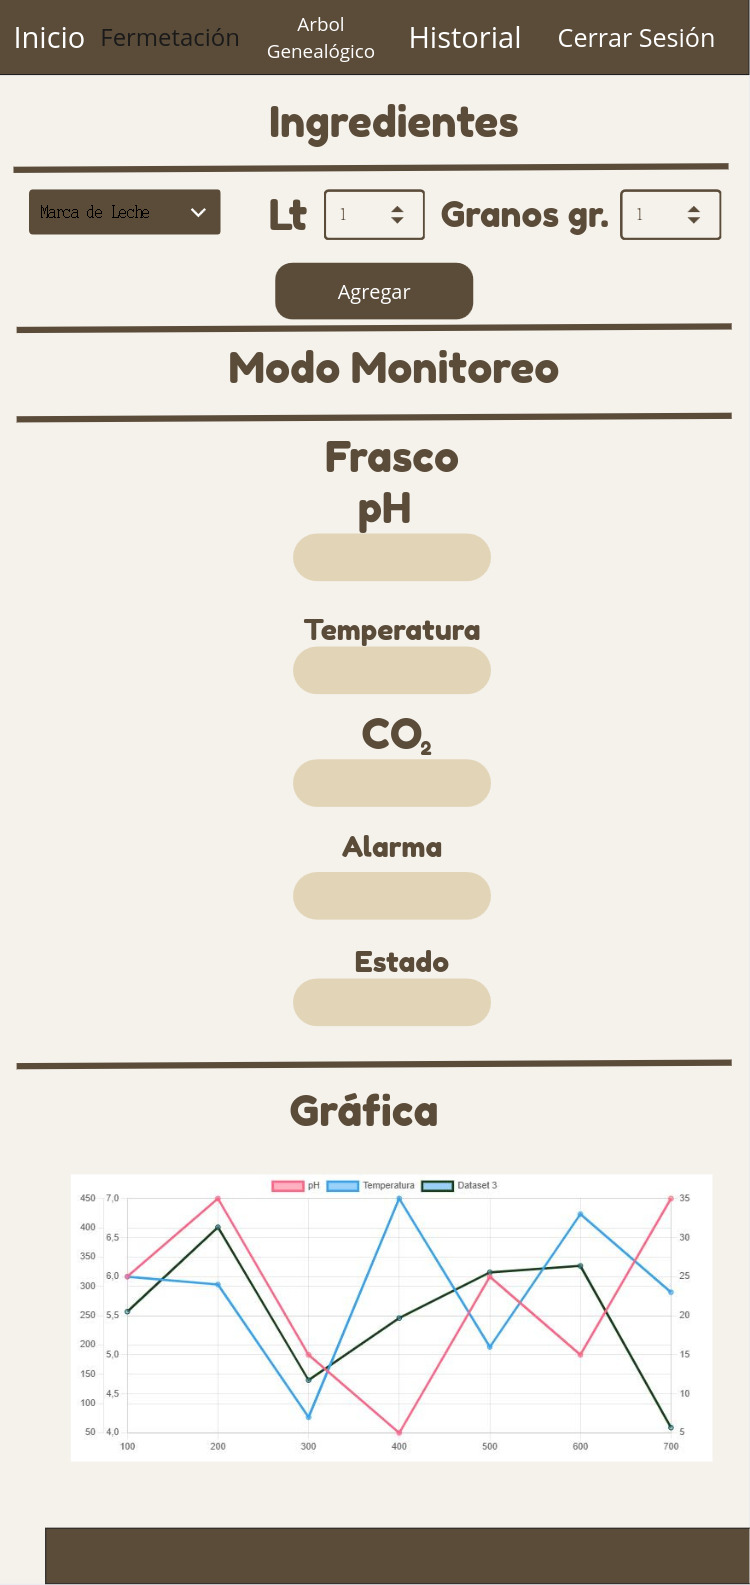
\includegraphics[width=0.6\textwidth]{./UML/Modulo4/Pagina/modomonitoreo.jpg}
\caption{Pantalla de monitoreo del productor inicial.}
\label{fig:MonitoreoInicial}
\end{figure} 

\begin{figure}[htb]
\centering
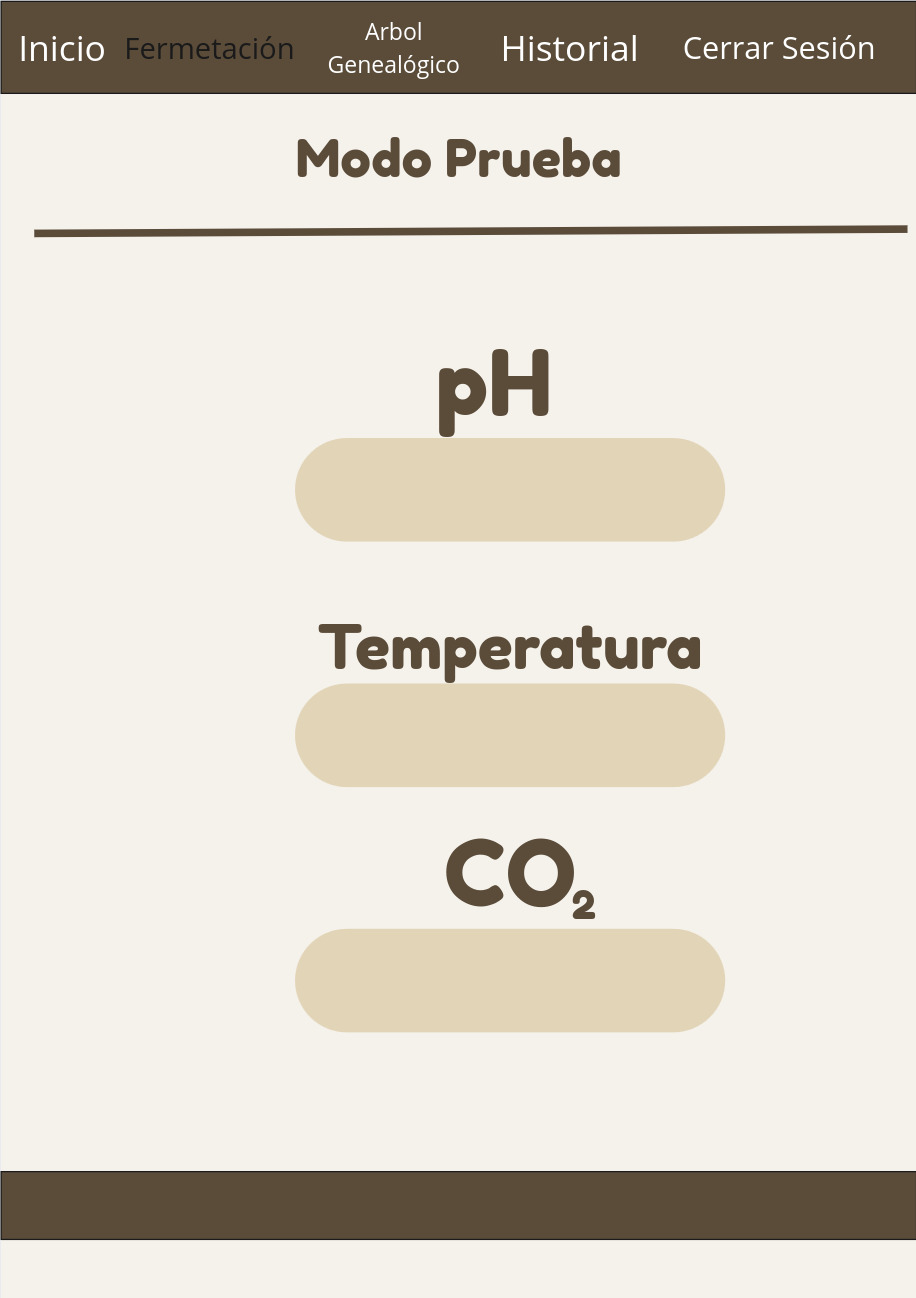
\includegraphics[width=0.5\textwidth]{./UML/Modulo4/Pagina/prueba.jpg}
\caption{Pantalla de prueba del productor inicial.}
\label{fig:PruebaInicial}
\end{figure} 

\begin{figure}[htb]
\centering
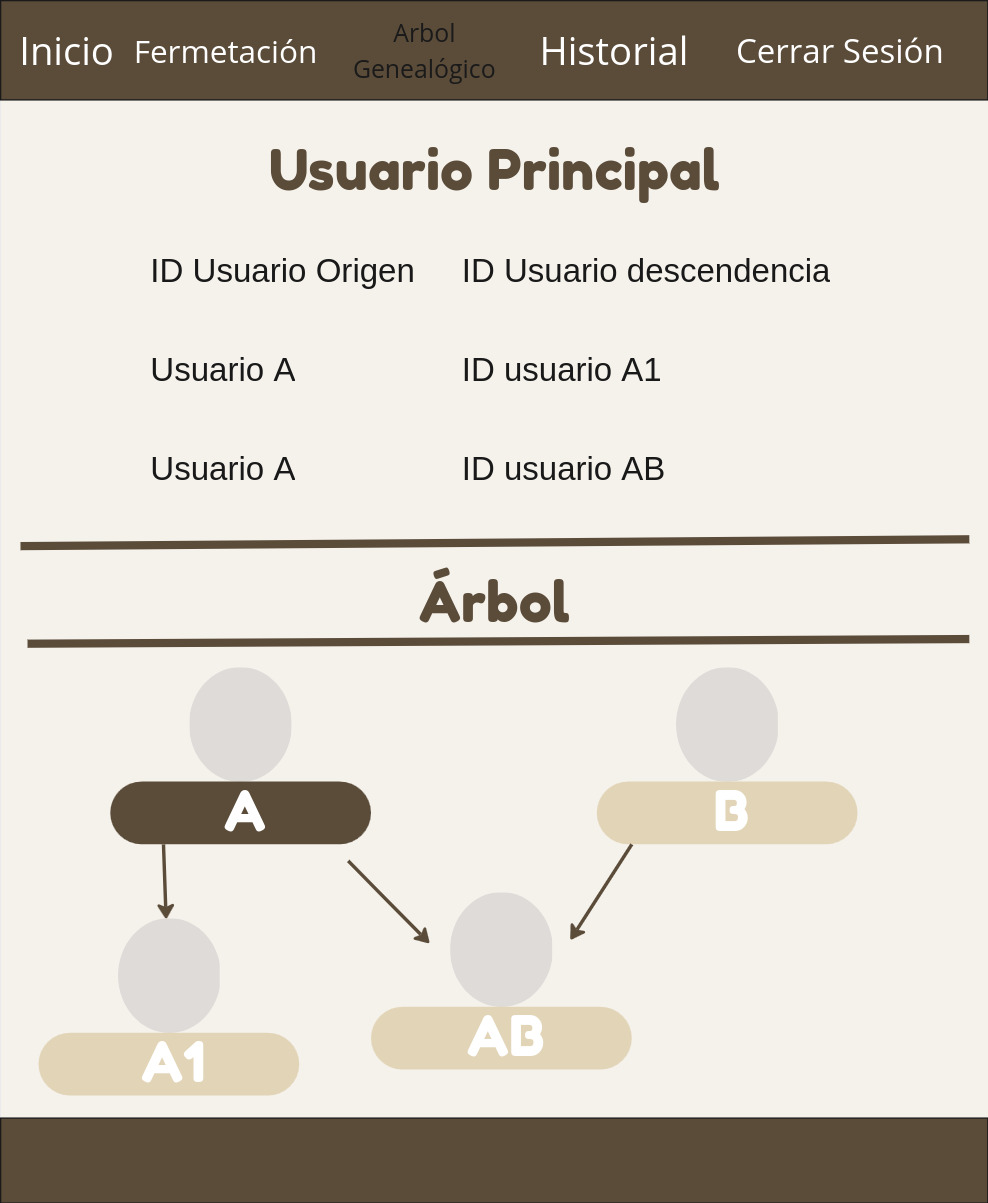
\includegraphics[width=0.5\textwidth]{./UML/Modulo4/Pagina/arbolprincipal.jpg}
\caption{Pantalla de árbol principal del productor inicial.}
\label{fig:ArbolPrincipal}
\end{figure} 

\begin{figure}[htb]
\centering
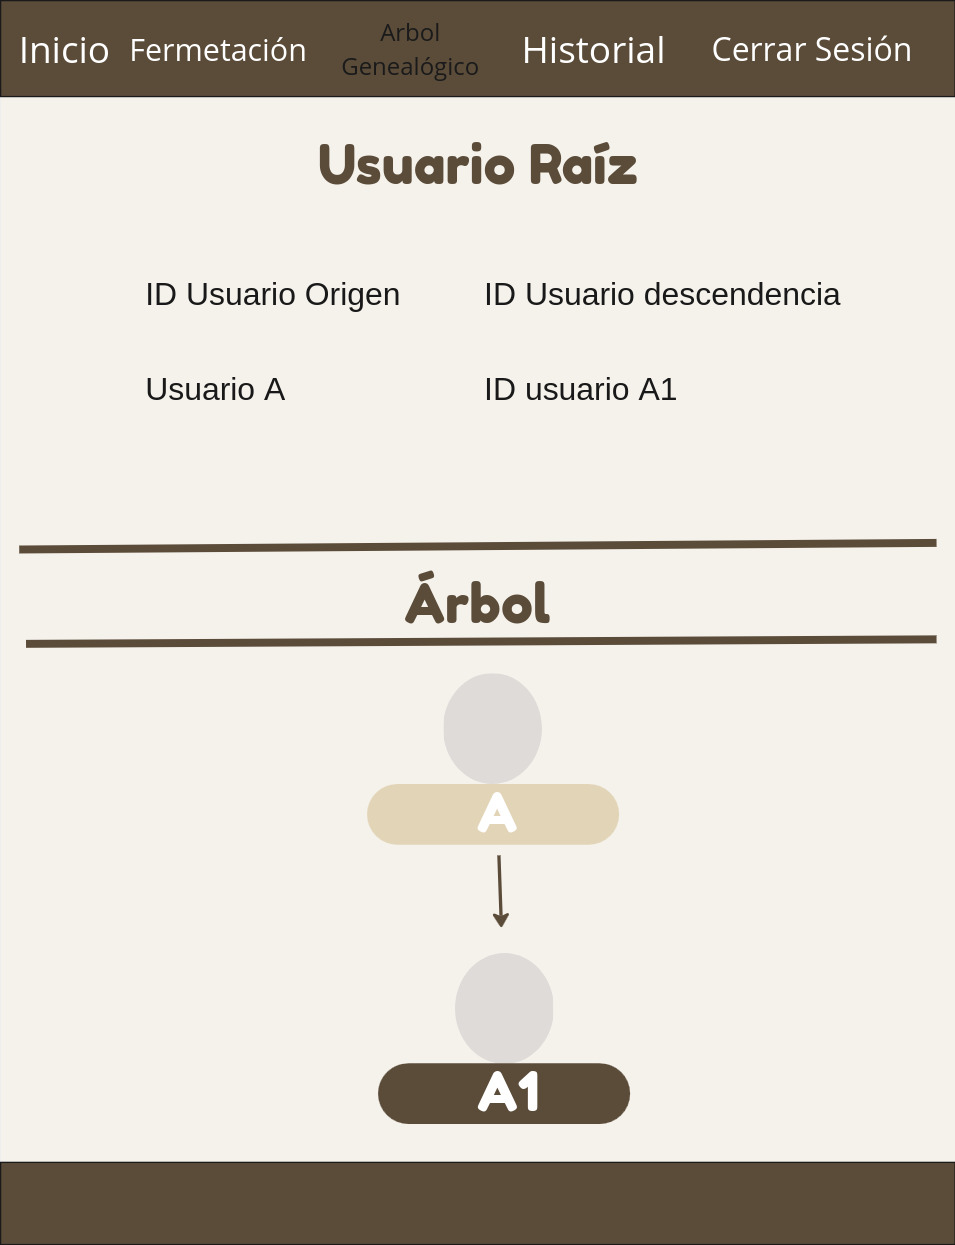
\includegraphics[width=0.5\textwidth]{./UML/Modulo4/Pagina/arbolraiz.jpg}
\caption{Pantalla de árbol raíz del productor inicial.}
\label{fig:ArbolRaiz}
\end{figure} 

\begin{figure}[htb]
\centering
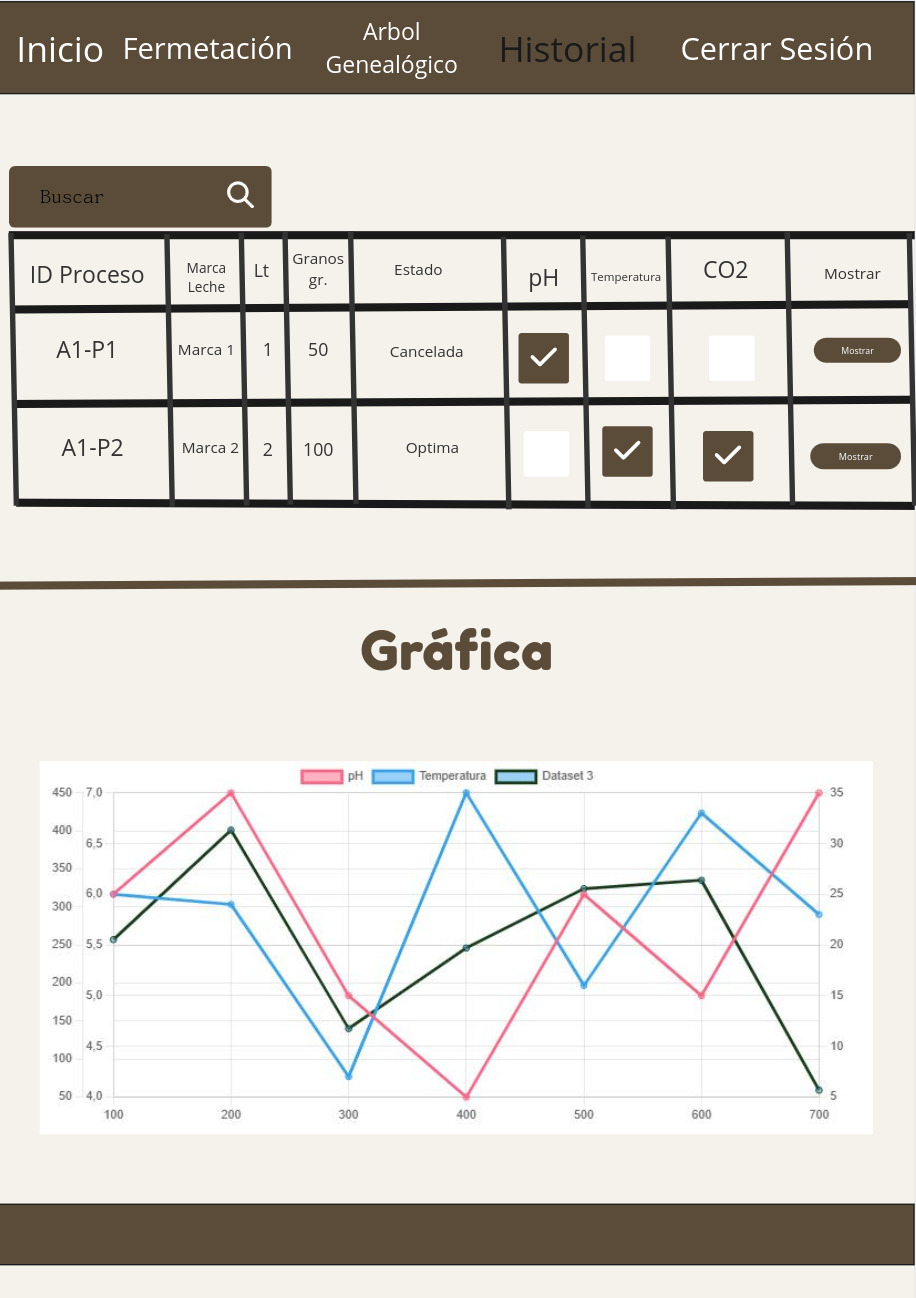
\includegraphics[width=0.5\textwidth]{./UML/Modulo4/Pagina/historial.jpg}
\caption{Pantalla de historial del productor inicial.}
\label{fig:Historial}
\end{figure} 

\subsubsection{Secuencia de páginas del Administrador}
Una vez que el administrador se autentica en el sistema, 
se despliega la pantalla de bienvenida mostrada en la \cref{fig:PrincipalAdmin}. 
Al acceder a la pestaña de procesos, se ilustran exclusivamente las fermentaciones activas
que se encuentran en modo de monitoreo, tal como se observa en la \cref{fig:ProcesosAdmin}. 

Posteriormente, al seleccionar la pestaña del árbol principal, 
se presenta la interfaz del árbol genealógico en la \cref{fig:ArbolAdmin}, 
la cual consolida la estructura de cada uno de los productores registrados. 
Asimismo, la pestaña de administración despliega la pantalla presentada en la \cref{fig:CRUDAdmin}, 
donde es posible llevar a cabo la actualización y eliminación de usuarios. 

En la pestaña de historial, ilustrada en la \cref{fig:HistorialAdmin}, 
el administrador puede consultar los registros históricos de todos los productores. 
Finalmente, al acceder a la pestaña de cuestionario, 
se despliegan las interfaces de la \cref{fig:CuestionarioInicial} y de la \cref{fig:CuestionarioRaiz}, 
diseñadas para la creación y registro de nuevos productores según su perfil (productor inicial o productor raíz).


\begin{figure}[htb]
\centering
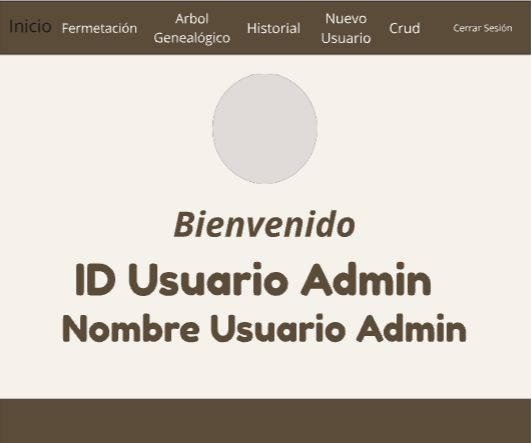
\includegraphics[width=0.8\textwidth]{./UML/Modulo4/Pagina/principaladmin.png}
\caption{Pantalla principal del administrador.}
\label{fig:PrincipalAdmin}
\end{figure} 

\begin{figure}[htb]
\centering
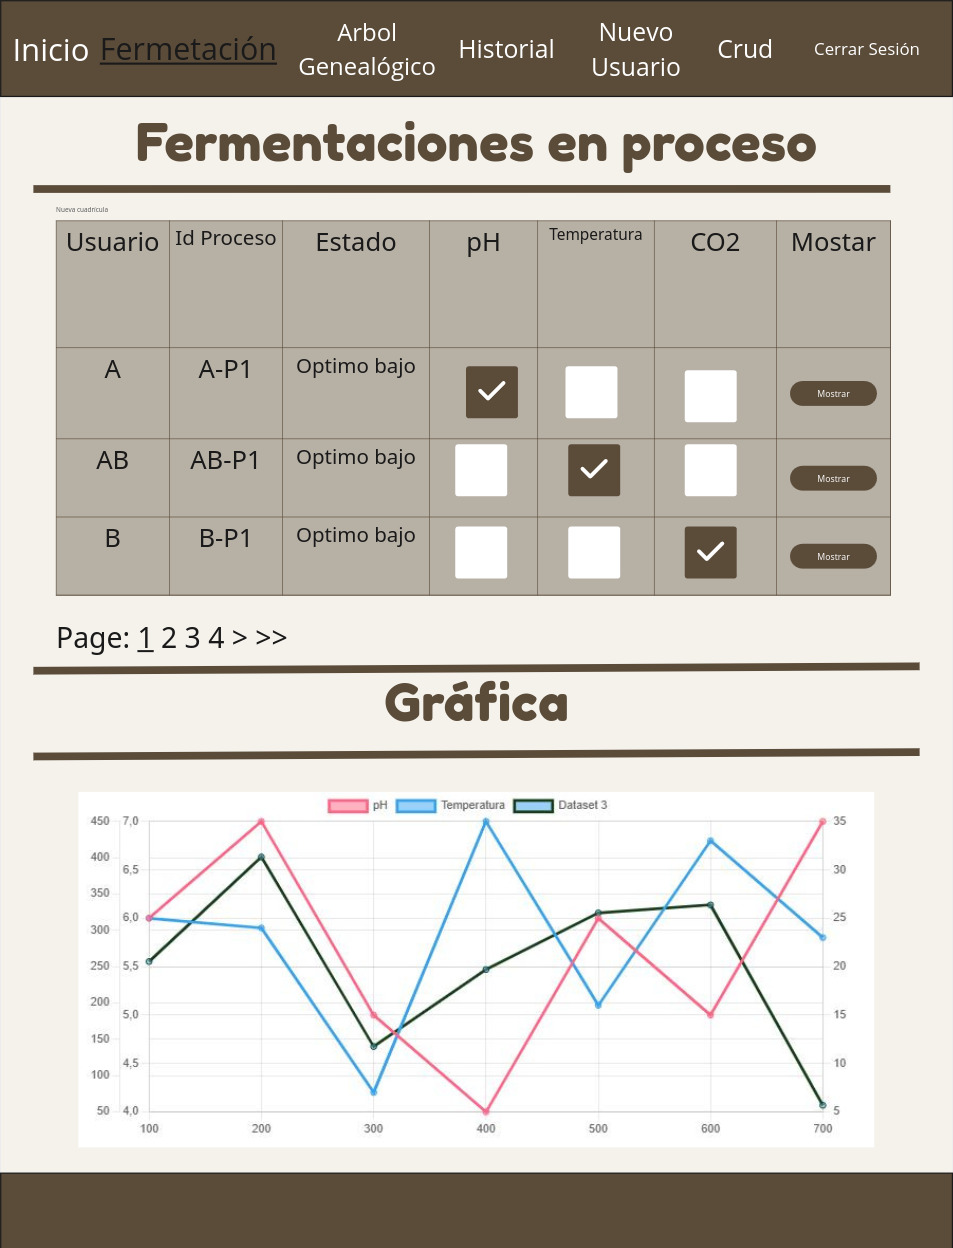
\includegraphics[width=0.5\textwidth]{./UML/Modulo4/Pagina/proceso1.jpg}
\caption{Pantalla de procesos del administrador.}
\label{fig:ProcesosAdmin}
\end{figure} 

\begin{figure}[htb]
\centering
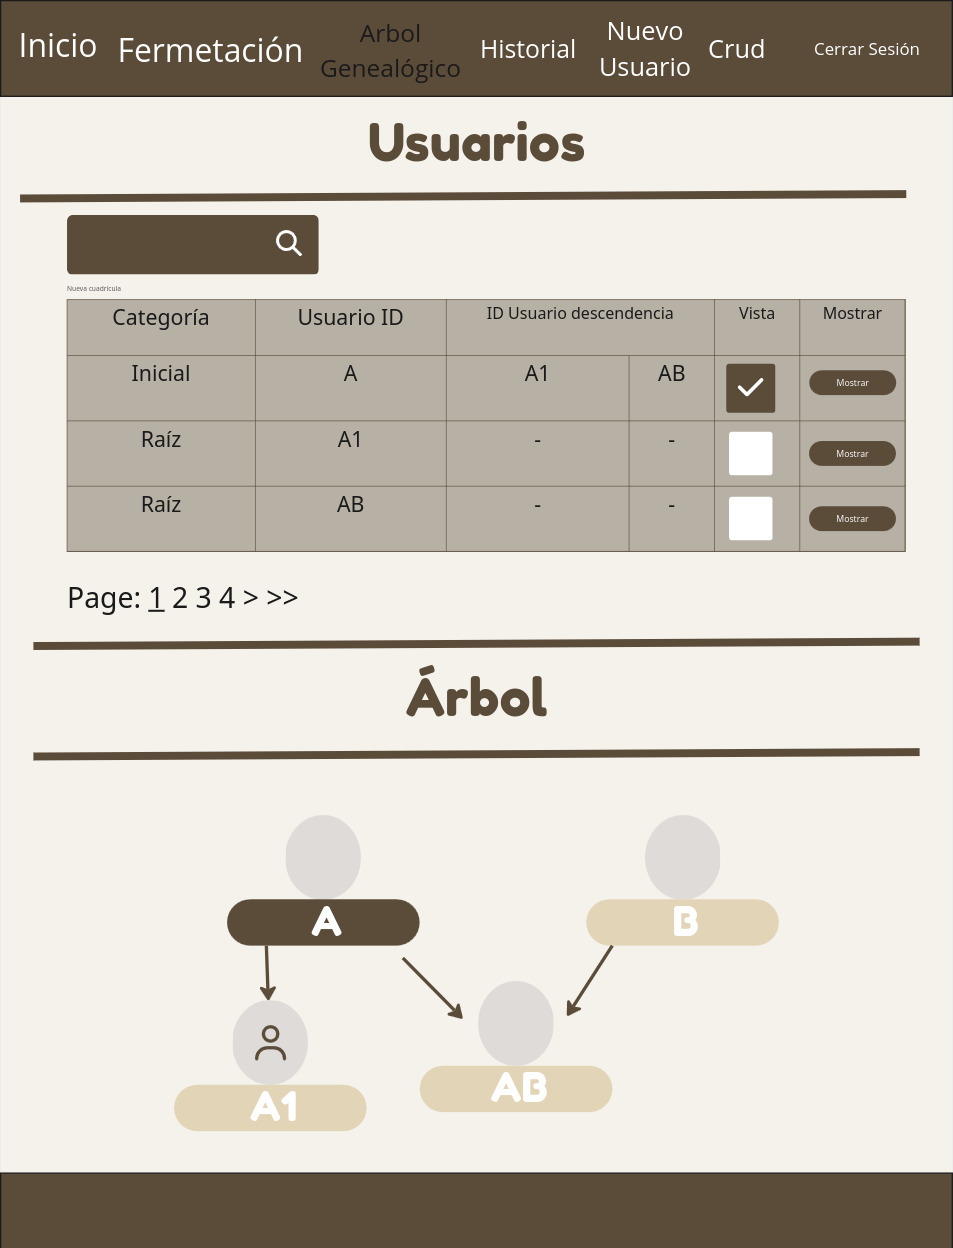
\includegraphics[width=0.5\textwidth]{./UML/Modulo4/Pagina/arboladmin.jpg}
\caption{Pantalla de árbol del administrador.}
\label{fig:ArbolAdmin}
\end{figure} 

\begin{figure}[htb]
\centering
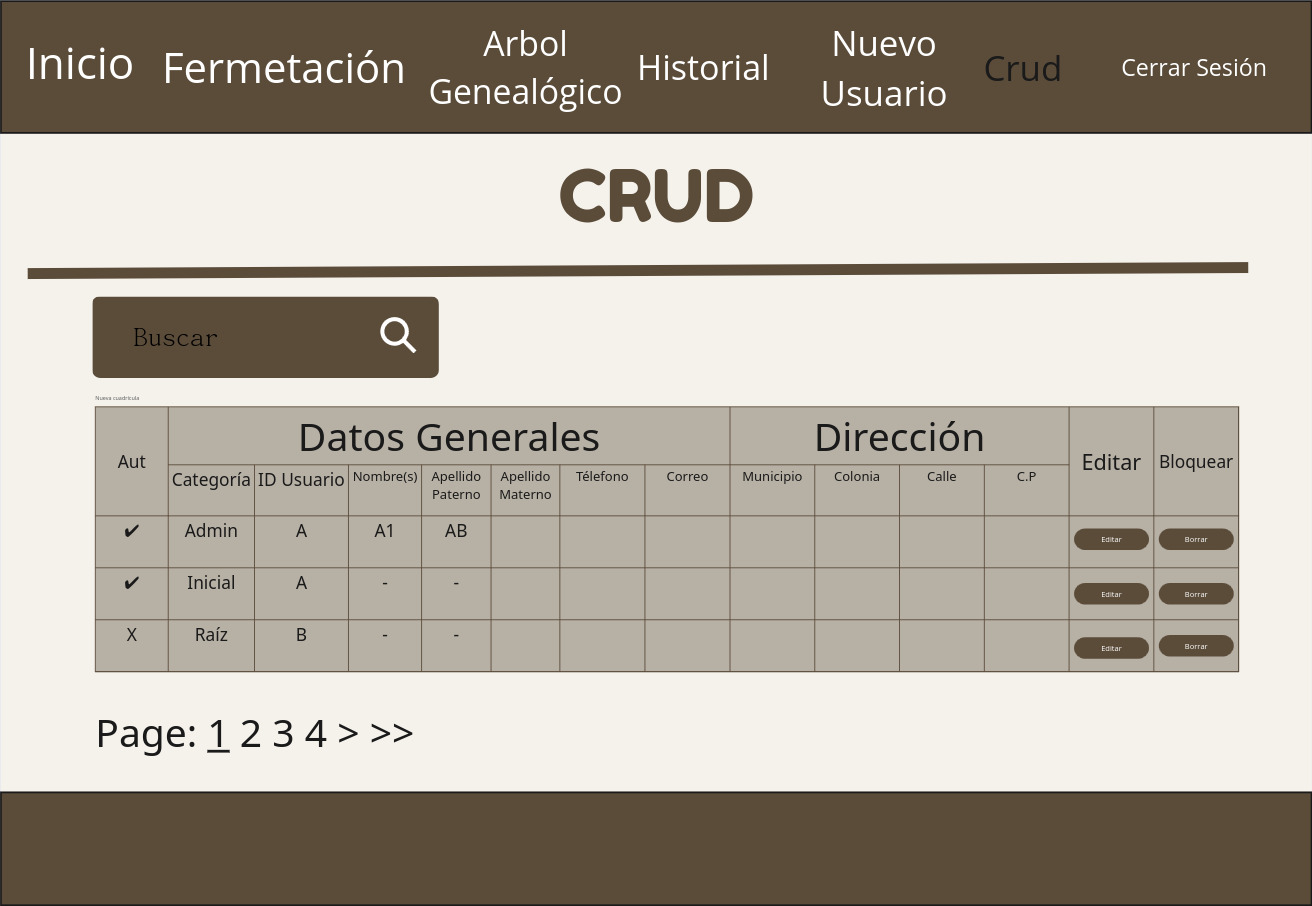
\includegraphics[width=0.5\textwidth]{./UML/Modulo4/Pagina/crud.jpg}
\caption{Pantalla de CRUD del administrador.}
\label{fig:CRUDAdmin}
\end{figure} 

\begin{figure}[htb]
\centering
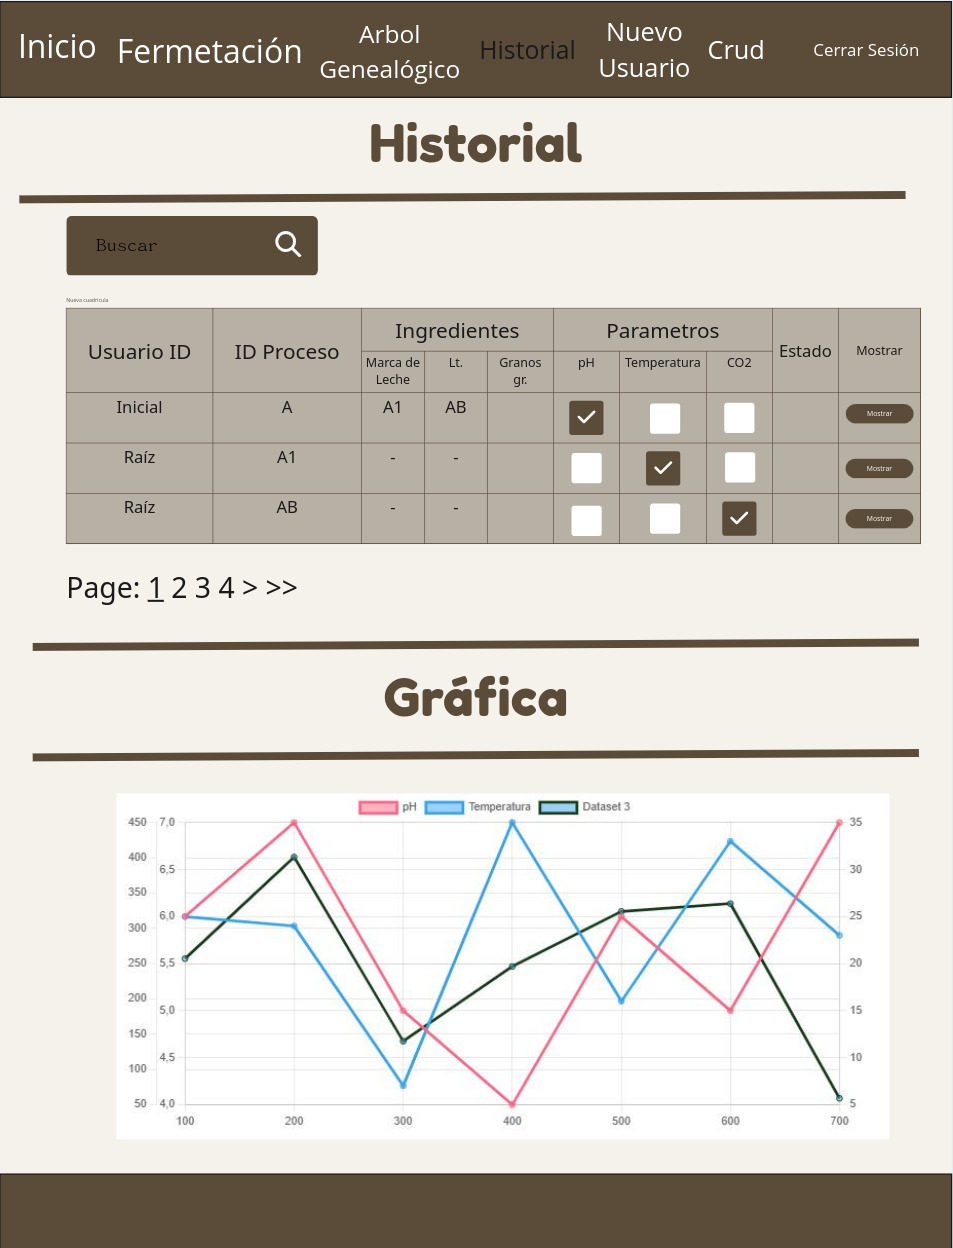
\includegraphics[width=0.5\textwidth]{./UML/Modulo4/Pagina/historialadmin.jpg}
\caption{Pantalla de historial del administrador.}
\label{fig:HistorialAdmin}
\end{figure} 

\begin{figure}[htb]
\centering
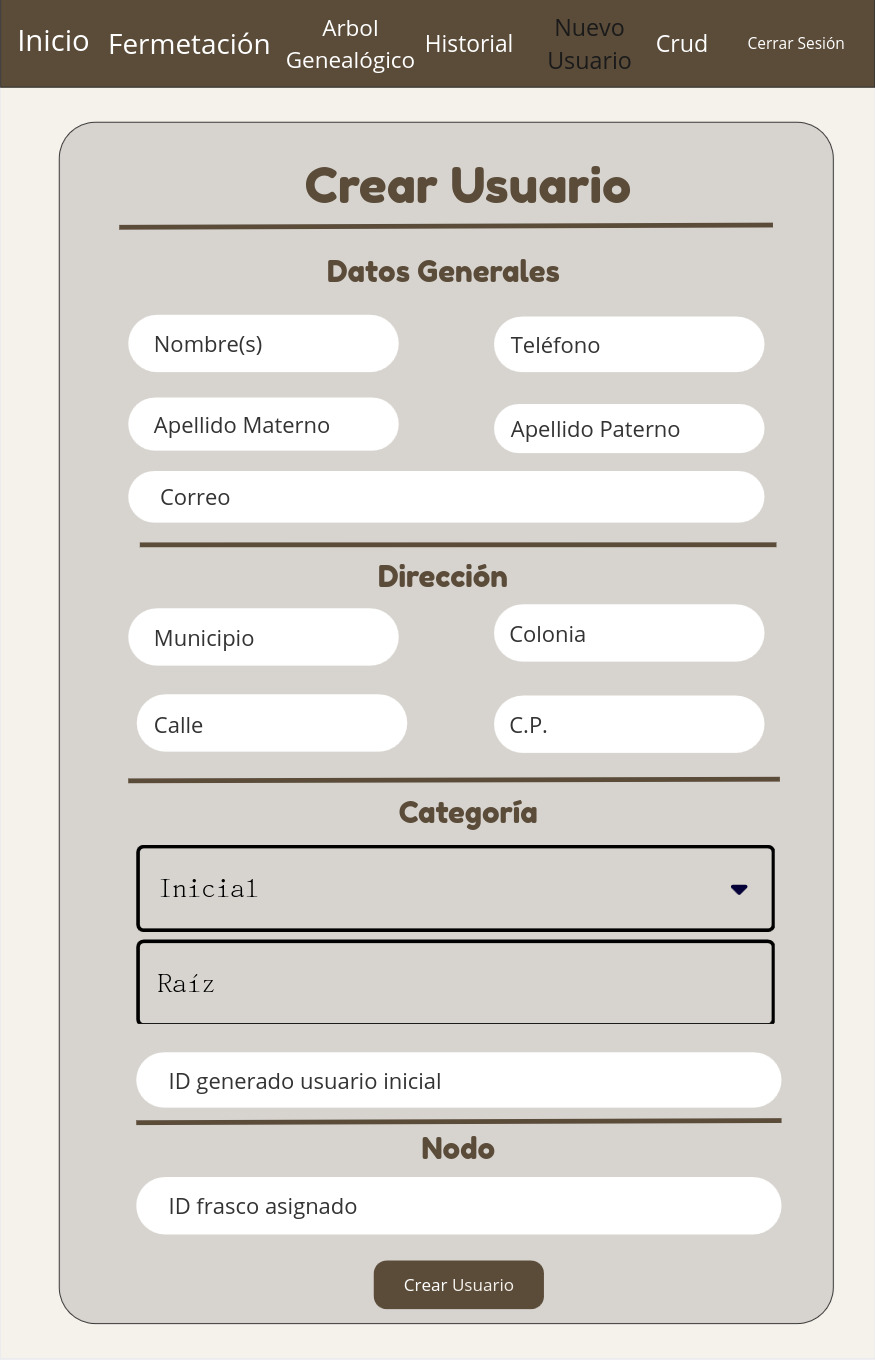
\includegraphics[width=0.5\textwidth]{./UML/Modulo4/Pagina/cuestionarioUsuarioInicial.jpg}
\caption{Pantalla de cuestionario del productor inicial.}
\label{fig:CuestionarioInicial}
\end{figure} 

\begin{figure}[htb]
\centering
\includegraphics[width=0.5\textwidth]{./UML/Modulo4/Pagina/cuestionariousuarioRaiz.jpg}
\caption{Pantalla de cuestionario del productor raíz.}
\label{fig:CuestionarioRaiz}
\end{figure} 